\documentclass{article}
\title{ゲーム理論入門 — 相手がいるときの判断の数学}
\author{TeX 図書館}

\begin{document}

\section{読み方 — この本の地図と 3 つの道具}

普段の判断は、天気や数字という「相手がいない問題」です。しかし値段の交渉、会議での発言、車の譲り合い、受験の併願には\textbf{相手の選択}が絡みます。自分の最善手が、相手の選び方によって変わる。こうした「相手がいるときの判断」を数理で扱うのが\textbf{ゲーム理論}です。

つまずきの原因は、ほぼ 1 つ。\textbf{「自分がどうしたいか」を考える前に、場面の構造を書き出していない}こと。ゲーム理論の道具はすべて、「誰が、何を選べて、それぞれの結果で何を得るか」を書き出した後に使います。書き出しが 8 割、計算は 2 割です。

\subsection{全 10 節の見取り図}

節の配分は次のとおりです。

\begin{enumerate}
\item 第 1 節: 読み方。道具を決めます。
\item 第 2〜3 節: 利得表とナッシュ均衡。場面を表にし、落ち着き先を読みます。
\item 第 4〜5 節: 囚人のジレンマと繰り返しゲーム。協力の難しさと、協力できる条件。
\item 第 6〜7 節: 混合戦略と展開形ゲーム。手を混ぜる、順番を考える。
\item 第 8〜9 節: 情報の非対称性と公共財。知らない相手、全員の問題。
\item 第 10 節: まとめと次の一歩。
\end{enumerate}

各節の終わりには\textbf{解答の指針}を置きます。答えの丸写しではなく、場面をどう書き出し、どの道具を当てはめるかを書く欄です。まず自力で 5 分考えてから、その欄を開いてください。

\subsection{本書で使う 3 つの道具}

道具は次の 3 つに絞ります。

\begin{itemize}
\item \textbf{利得表}: プレイヤー・戦略・結果の満足度を 1 枚の表に書いたもの。
\item \textbf{均衡}: 全員が自分の戦略に満足して、誰も動きたくない状態。
\item \textbf{後ろ向き帰納}: 順番があるゲームでは、終わりから逆にたどる解き方。
\end{itemize}

\begin{quote}
\textbf{【注意】}\ ゲーム理論の「ゲーム」は勝ち負けの遊びのことではありません。\textbf{相手の選択が自分の結果に影響する、あらゆる場面}のことです。そして利得は金額ではなく「その人の主観的な満足度」です。相手の利得を勝手に自分基準で見積もるのが、実務での最大の誤りです。
\end{quote}

\textbf{解答の指針:}\ どんな場面でも、まず「プレイヤーは誰か」「各人は何を選べるか」「結果ごとに何が得られるか」の 3 行を書く。これで利得表か展開形(順番あり)かが見え、使う道具が決まります。問題文を読みながら頭の中だけで結論を出そうとしないこと。書き出した表が、そのまま答えの材料になります。

\section{利得表 — 場面を 1 枚の表にする}

最初の道具は\textbf{利得表}です。2 人のプレイヤーが同時に手を選ぶ場面は、次の形の表に書けます。行は自分の選択肢、列は相手の選択肢で、ます目にはその結果で両者が得るものを並べます。

\[ (自分の利得, 相手の利得) \]

例として、2 人でドライブに行くか映画に行くか選ぶ場面(「男女のケンカ」の古典例)を考えます。どちらか一方でも我慢すれば一緒にいられますが、別行動はつまらない、という場面です。表にすると次のようになります。

\begin{itemize}
\item 両方がドライブ: (3, 2)。自分はドライブが好き、相手はまあ満足。
\item 両方が映画: (2, 3)。逆の好み。
\item 別行動: (0, 0)。どちらもつまらない。
\end{itemize}

\begin{figure}
\centering
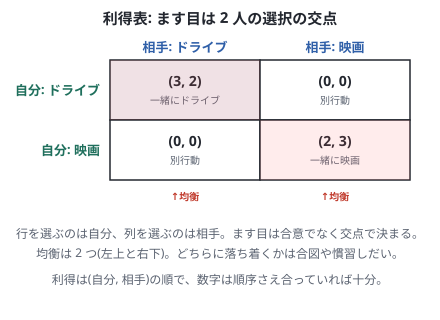
\includegraphics[width=0.85\textwidth]{figures/payoff-matrix.svg}
\caption{利得表の例: ます目には(自分, 相手)の利得を並べる}
\end{figure}

この表の読み方の核心は、\textbf{「ます目を選ぶのは 2 人の合意ではない」という点}です。自分は行を選び、相手は列を選ぶ。結果のます目は、2 人の選択の交点として勝手に決まります。だから「お互いに一番いいます目」があるとは限らないのです。

\subsection{最善応答: 相手の手が決まったら}

自分の選び方を評価する基準は\textbf{最善応答}です。「相手がこの列を選ぶなら、自分はこの行が一番」という対応のこと。利得表の各列に対して、一番利得の高い行に印を付けます。相手も同じように、各行に対して最善の列に印を付けます。

この 2 種類の印が\textbf{同じます目で重なった}とき、その組み合わせは特別な意味を持ちます。誰も自分の選択を変える理由がない状態、つまり次節のナッシュ均衡です。

\begin{quote}
\textbf{【注意】}\ 利得を書くときは、自分の好みの全順序が入るようにする。同点だらけの表は場面の把握が甘いサインです(本当に同点な場合は除く)。また、表に書くのは「結果の自分にとっての価値」であって、道徳的正当性ではありません。理論は価値の大きさを扱うだけで、何を良しとすべきかは教えません。
\end{quote}

\textbf{解答の指針:}\ 場面が与えられたら、(1) プレイヤー 2 人の名前を書く、(2) 各人の選択肢を 2〜3 個に絞る、(3) すべての組み合わせの結果を想像して利得を(自分, 相手)の順で書く。数字は絶対的なものでなくてよく、順序が正しければ十分です(満足 3 と 2 は、3 のほうが良いことだけを意味します)。絞り込みに迷ったら、最も極端な 2 択から始めます。

\section{ナッシュ均衡 — 誰も動きたくない状態}

\textbf{ナッシュ均衡}とは、\textbf{全員が自分の戦略に満足していて、他の人の選択は変わらないという前提のもとで、誰も自分の選択を変えようとしない状態}です。最善応答が全員について重なったます目のことでした。

定義の読み方に注意します。「みんなにとって一番いい状態」ではありません。\textbf{「動くと損をする、だから動かない」状態}です。この 2 つは全く別で、均衡が非効率な場面を扱うのが第 4 節の囚人のジレンマです。

\subsection{ケンカの例: 均衡は 2 つ}

前節のドライブ・映画の表には、均衡が 2 つあります。(ドライブ, ドライブ)では自分は最善(3)、相手は最善(2)なので誰も動きません。(映画, 映画)でも同様です。別行動のます目は、どちらも別の選択に変えると利得が上がるので均衡ではありません。

\textbf{均衡が複数ある}ことは、実務で非常に重要です。均衡が 1 つなら場面は勝手にそこへ向かいますが、複数ある場合、どの均衡に落ち着くかは\textbf{合図・慣習・交渉}で決まります。待ち合わせ場所が決まらないのは均衡が複数だからで、「いつもの場所」という慣習は均衡を選ぶ装置です。

\subsection{均衡がないように見える場面}

じゃんけんのように、どの組み合わせでも「負けた側が手を変えたくなる」場合は、純粋な(1 つの手に固定した)均衡が存在しません。この場合でも、\textbf{手をランダムに混ぜる}と均衡が作れることが知られています。これが第 6 節の混合戦略です。

ナッシュ均衡の存在定理は「有限なゲームには必ず均衡がある(混合戦略を許せば)」という強い結果で、この理論の土台です。だから、均衡が見つからないと感じたら、それは「手を混ぜる」可能性を見落としているサインです。

\begin{quote}
\textbf{【注意】}\ 均衡は予測の道具であって、望ましい状態の保証ではありません。「均衡だから正しい」という議論は誤りです。均衡は単に「そこに落ち着くと誰も動かない」と言うだけで、そこに至る経路や、他の均衡のほうが全員にとって良いこともあります。
\end{quote}

\textbf{解答の指針:}\ 利得表が書けたら、(1) 自分の各列に対する最善応答の行に印を付け、(2) 相手の各行に対する最善応答の列に印を付け、(3) 印が交差するます目をすべて書き出す。これが均衡の候補です。均衡が複数出たら、どれに落ち着きやすいか(合図や慣習があるか)を一言で書き添える。見つからなければ混合戦略(第 6 節)を疑います。

\section{囚人のジレンマ — なぜ協力は難しいのか}

最も有名な場面を扱います。2 人の共犯者が別々の部屋で尋問されます。お互いに黙秘すれば軽い刑、一方が裏切れば裏切り者は釈放・黙秘者は重い刑、両方が裏切れば中くらいの刑。利得(良いほうが大きい)で書くと次のとおりです。

\begin{itemize}
\item 両方協力(黙秘): (3, 3)。全体として最も良い。
\item 自分だけ裏切り: (5, 0)。自分にとって最高。
\item 相手だけ裏切り: (0, 5)。自分にとって最悪。
\item 両方裏切り: (1, 1)。
\end{itemize}

\begin{figure}
\centering
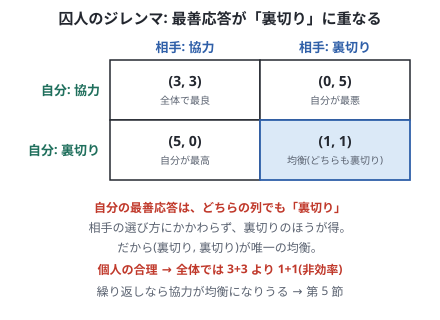
\includegraphics[width=0.85\textwidth]{figures/prisoners-dilemma.svg}
\caption{囚人のジレンマ: 最善応答が「裏切り」に重なる}
\end{figure}

\subsection{なぜ裏切りが最善応答なのか}

相手が黙秘するなら、自分は黙秘(3)より裏切り(5)のほうが得。相手が裏切るなら、自分は黙秘(0)より裏切り(1)のほうがまし。\textbf{相手の選び方にかかわらず、裏切りのほうが得}。だから裏切りが最善応答で、(裏切り, 裏切り)が唯一の均衡です。

しかし全体では(協力, 協力)の 3+3 のほうが 1+1 よりずっと良い。\textbf{個人の合理性が、全体にとって最悪に近い均衡へ導く}。これがジレンマの正体です。日常のいたる所がこの構造をしています: 遅刻しない代わりに手を抜く全員の事情、公害を出す工場、値段競争に突入する会社、会議の発言を控える全員。

\subsection{1 回きりと、繰り返しの違い}

1 回だけの取引なら、ジレンマの均衡は裏切りです。しかし\textbf{同じ相手と何度も会う}場合は話が変わります。裏切った相手とは次から協力してもらえない。\textbf{未来の利益が、現在の裏切りの誘惑に勝てば、協力が均衡になる}のです。この条件を扱うのが第 5 節です。

\begin{quote}
\textbf{【注意】}\ ジレンマの構造を見抜くポイントは、「自分だけ裏切り」が最高で「両方裏切り」がまし、という利得の順序です。この順序が崩れると別のゲームになります。場面がジレンマかどうかは、この 4 つの利得の順序を確認すれば判定できます。
\end{quote}

\textbf{解答の指針:}\ 「これはジレンマか?」という問題では、(1) 4 つのます目の利得を順序付きで書く、(2) 「自分だけ裏切りが最高・両方裏切りが 2 番目」の順序かを確認する、(3) 均衡が裏切りと裏切りの交点であることを最善応答で確かめる。実例(環境・価格競争・共有リソース)に当てはめるときは、「協力」「裏切り」に相当する行動を日本語で書き直してから表にします。

\section{繰り返しゲーム — 明日があれば協力できる}

1 回きりのジレンマでは裏切りが均衡でしたが、同じ場面が何度も続く(\textbf{繰り返しゲーム})と、協力が安定的に成り立ちます。鍵は\textbf{将来の関係への評価}です。

\subsection{しっぺ返し戦略}

有名な戦略が\textbf{しっぺ返し}(Tit for Tat)です。ルールはシンプルで、「最初は協力し、以後は相手が前回やったことをする」。相手が協力すれば協力、裏切れば 1 回だけ裏切りで応じます。

この戦略が強い理由は 2 つです。\textbf{寛容}(先に手を出さない)と、\textbf{報復の確実さ}(裏切りを見逃さない)です。コンピュータ大会で最初期に優勝して以来、「シンプルに見えて強い協力戦略」の代表例として研究されてきました。良い戦略の条件は、賢さではなく\textbf{予測しやすさ}にある、という直感に反する発見です。

\subsection{協力が成立する条件: 未来の重み}

繰り返しゲームで協力が均衡になる条件は、\textbf{「次の関係が続く可能性が十分高い」}ことです。裏切りで 1 回得をしても、その後協力が崩れて損する分のほうが大きければ、裏切りは得になりません。逆に、\textbf{関係がもうすぐ終わる}と分かっているなら、裏切りが均衡に戻ります(最終回の前で裏切る誘惑、いわゆる「終わりの問題」)。

この視点は実務に直結します。長期的な取引先との関係で手抜きが少ないのは、しっぺ返しと未来の重みが効いているからです。逆に、一度きりの観光地の店でトラブルが起きやすいのは、\textbf{繰り返しが期待できない場面}だからです。仕組みを知れば、行動の予測ができます。

\begin{quote}
\textbf{【注意】}\ しっぺ返しは万能ではありません。相手の裏切りを誤認すると、報復の連鎖(二重の誤解)に入る弱点があります。実務の教訓は「報復は 1 回にとどめ、誤解を解く窓口を用意する」という形で表現できます。
\end{quote}

\textbf{解答の指針:}\ 繰り返しの問題では、(1) 1 回あたりの利得(協力 3、裏切り 5 など)を書く、(2) 「裏切って得た 1 回分」と「その後失う協力の流れ」を比べる、(3) 続く確率が高いほど協力が有利になることを確認する。戦略を評価するときは、寛容さ(先に裏切らない)と報復の確実さ(裏切りを見逃さない)の 2 軸で書くと整理しやすくなります。

\section{混合戦略 — 手を混ぜる均衡}

相手に読まれると損をする場面(じゃんけん、ペナルティーキック、検査の抜き打ち)では、\textbf{手をランダムに混ぜる}のが最善になります。\textbf{混合戦略}は、各手に確率を割り当てた戦略です。

\subsection{読まれないことが価値になる}

ペナルティーキックを考えます。蹴り手は左か右、キーパーも左か右に跳ぶ。蹴り手が「左が得意だからいつも左」なら、キーパーは左へ跳び続ければよい。\textbf{決め打ち(純粋戦略)は相手に利用される}ので、蹴り手は自分でもどちらに蹴るか決めず、確率で混ぜる必要があります。

均衡の確率は「\textbf{相手の混ぜ方が、自分のどちらの手でも利得が同じ}」という条件から決まります。片方の手が得なら、自分はその手に寄せてしまい、相手はそれに合わせて確率を変える。釣り合うまで確率が調整された点が均衡です。この「無差別条件」は計算の型として覚えられます。

\subsection{ランダムに見えることの難しさ}

人間が自力で作るランダムは偏ります(連続を避けすぎる、交代を好む)。実際のスポーツデータでは、プロのサーブやキックの配置が均衡の確率に近いことが確認されており、\textbf{訓練と経験が「疑似ランダムの質」を上げている}と解釈できます。日常の応用としては、抜き打ち検査やランダムな監査は「予測できる頻度」では効果が消える、という教訓が得られます。

\begin{quote}
\textbf{【注意】}\ 混合戦略は「迷い」ではありません。\textbf{読まれないために意図的に入れる不確実性}です。相手に読まれるコストが存在しない場面では、混合する必要はまったくありません。道具を使うかどうかは「読まれると損か」で判断します。
\end{quote}

\textbf{解答の指針:}\ 混合戦略の問題では、(1) 2 手の場合、相手が確率 \( p \) で手 A を出すと書き、(2) 自分の手 A と手 B の期待利得を \( p \) の式で書く、(3) 両者を等しいと置いて \( p \) を解く。これが均衡の混合比です。意味の確認として、「自分の混合比は相手の利得を等しくするために選ぶ」ことを一言で書き添えると、計算と概念がつながります。

\section{展開形ゲーム — 順番があるときは後ろから}

ここまでの手は同時選択でした。しかし交渉・入札・クイズのように\textbf{順番}がある場面では、\textbf{展開形}(ゲームの木)が自然な書き方です。分岐点(誰が選ぶか)と枝(選択肢)と葉(結果の利得)で描きます。

\subsection{後ろ向き帰納: 終わりから解く}

順番があるゲームの解き方は\textbf{後ろ向き帰納}です。最後の分岐点から見て、その時点で選ぶ人が選ぶ手を確定させ、その結果を 1 つ前の分岐点に持ち上げ、順に手前まで解いていきます。

例: 店(先手)が「安売りする / しない」を選び、次に競合店(後手)が「値下げで対抗 / しない」を選ぶ場面。対抗して両方が潰し合うより、しないほうが競合店にとって良いなら、後手の選択は「しない」に確定します。すると先手は「後手は対抗しない」を前提に判断できる。\textbf{先手は、後手の反応を先読みして初手を決められる}のが、順番があることの利点です。

\begin{figure}
\centering
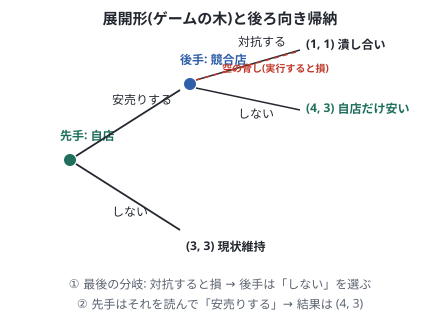
\includegraphics[width=0.85\textwidth]{figures/game-tree.svg}
\caption{展開形: 終わりの分岐から逆にたどる(後ろ向き帰納)}
\end{figure}

\subsection{脅しが信じられるか: 威嚇の条件}

後ろ向き帰納の教訓は、\textbf{「脅しは実行する意思がなければ効かない」}です。後手が「対抗してやる」と言っても、実際に対抗すると損なら、先手はそれを織り込んで判断します。空の脅しは均衡に影響しない。\textbf{脅しを効かせるには、実行するのが自分にとっても最善になる仕組み}を先に作っておく必要があります(約束の公開、評判、法的拘束など)。

\begin{quote}
\textbf{【注意】}\ 展開形を利得表(同時選択の形)に直すときは、後手が先手の手を知ったうえで選ぶという違いが消えます。順番の情報は、均衡を変える重要な要素です。「同時に選ぶか、順番に選ぶか」を最初に確認する習慣をつけてください。
\end{quote}

\textbf{解答の指針:}\ 順番がある問題では、(1) ゲームの木を分岐順に描く(各分岐に「誰が選ぶか」を書く)、(2) 最後の分岐から、選ぶ人にとって最善の枝に印を付ける、(3) 印の付いた結果を 1 つ前の分岐の利得として引き上げ、手前まで繰り返す。脅しや約束が話題に出たら、「その行動が実際に最善か」を各分岐で確認するのが後ろ向き帰納の読み方です。

\section{情報の非対称性 — 知っている側と知らない側}

売り手は品物の質を知っているが買い手は知らない。労働者は自分の能力を知っているが雇用主は知らない。\textbf{持っている情報が違う}場面は、この本で扱う中で最も実務に近い題材です。

\subsection{レモン市場: 良い品が消える仕組み}

有名な中古車の例(レモン市場)を考えます。車には良い車(良品)と悪い車(不良品)があり、売り手だけがどちらかを知っています。買い手は「平均的には半々」と知っているだけなので、\textbf{平均の価値しか払わない}。

すると、良品の売り手は平均価格では割に合わず、市場から良品が抜けます。抜けた結果、平均はさらに下がり、次に良い品が抜ける。\textbf{情報の非対称性が、良い品を市場から駆逐していく}連鎖です。これは市場の失敗の代表例で、誰かが悪意あるからではなく、\textbf{価格が平均に釣り合うという仕組みそのもの}が原因です。

\subsection{シグナリングとスクリーニング: 信じられる合図}

この問題への対処が、\textbf{信じられる合図}です。良い品の売り手だけがコストを払える合図(長期保証、実績の公開、資格取得)は、不良品の売り手にはまねができないので、質を区別する装置になります。\textbf{まねができないからこそ、合図として機能する}のが理論上の核心です。

学歴や資格が就職の場面で機能するのも同じ構造です。能力を直接測れない雇用主に対して、取れる人だけが取れる資格が\textbf{能力の合図}として働きます。買い手側が仕組みを作る形(\textbf{スクリーニング})では、面接や試用期間で「分かれる場面」を用意します。

\begin{quote}
\textbf{【注意】}\ 合図は「派手さ」ではなく\textbf{「まねコストの差」}で選びます。誰でも出せる合図は情報を持たず、場面だけが騒がしくなります。合図を設計・評価するときは、「これは不審者が出せないものか」を必ず問うてください。
\end{quote}

\textbf{解答の指針:}\ 情報の非対称の問題では、(1) 誰が何を知っていて、誰が何を知らないかを 2 行で書く、(2) 知らない側が平均で判断すると何が起こるか(良い品が抜ける連鎖)をたどる、(3) 対処は「まねができるか」で評価する。保険や中古市場、採用の問題はすべて同じ手順で書けます。「知らない側の平均判断」を書き出すのが出発点です。

\section{公共財と社会的ジレンマ — 全員の問題}

最後の道具は、プレイヤーが 2 人ではなく\textbf{多数}になる場面です。誰もが使える公共の資源(道、空気、漁場、オープンソースの維持)は、全員が少しずつ払えば作れるのに、\textbf{自分だけ払わずに便乗する}(フリーライド)誘惑が常にあります。

\subsection{ジレンマの連鎖は全員版ジレンマ}

公共財の実験(実際に人を集めて行う経済実験)では、最初は多くの人が払うのに、繰り返すうちに払う人が減っていく、というパターンが安定して観察されます。\textbf{裏切りを見つけられない・罰せられない}構造では、協力が減っていくからです。しかし、\textbf{フリーライダーを罰するコストを自分で払える}仕組みを入れると、協力が回復します。罰の有効性は、多数の場面でのしっぺ返しの一般形と読めます。

\subsection{制度がゲームを変える}

ゲーム理論の実務的な教訓は、\textbf{人の心を変えるより、利得表を変える}ほうが効く、というものです。自動回収のゴミ箱、使うと記録される駐車場、貢献が見える名前つきのコミットログ。\textbf{構造を 1 か所変えると、各人の最善応答が変わり、均衡が移動します}。第 6 節の社会心理の教訓(心がけより構造)と同じ結論に、利得表の言葉でたどり着きます。

\begin{quote}
\textbf{【注意】}\ 「全員が協力すればみんな得」を知らせるだけでは、公共財問題は解けません。知っていてもフリーライドが最善応答のままだからです。解けるのは、協力する人の利得が上がる、または裏切る人の利得が下がる\textbf{仕組み}を入れたときだけです。
\end{quote}

\textbf{解答の指針:}\ 公共財の問題では、(1) 払う / 払わない(または提供する / 便乗する)の 2 択を全員分で書き、(2) 自分だけ払わなかった場合の利得と、全員が払わなかった場合の利得を比べる、(3) 「自分 1 人の裏切りが全体の均衡を壊す」連鎖を確認する。対策を考える問題では、罰(コスト)・可視化(記録)・繰り返し(関係の継続)の 3 つが利得表のどこを動かすかを書きます。

\section{まとめと次の一歩}

9 節を振り返ります。道具は、実は 5 つしかありません。

\begin{itemize}
\item \textbf{利得表}: 誰が・何を選べる・何を得るかを 1 枚に。分析の出発点。
\item \textbf{ナッシュ均衡}: 誰も動きたくない点。複数あることも、非効率なこともある。
\item \textbf{繰り返し}: 未来の重みが協力を作る。しっぺ返しはシンプルに強い。
\item \textbf{後ろ向き帰納}: 順番があるなら終わりから。空の脅しは均衡に効かない。
\item \textbf{情報と制度}: まねできない合図が信頼を作り、利得表の変更が行動を変える。
\end{itemize}

ゲーム理論の学習で一番効くのは、\textbf{身のまわりの場面を利得表に書き直すこと}です。会議の発言、家の分担、店の値段設定。読んだ節のたびに 1 つの場面を選び、3 行で書き出して均衡を読んでください。理論は「分かった気」になりやすい科目ですが、自分の場面で均衡が 1 つ書けるかどうかで理解の質が全く変わります。

次の一歩としては、この本の先は次のような本へつながります。

\begin{itemize}
\item 均衡の確率の計算を深く → \textbf{統計学入門}(期待値と確率の道具箱です)
\item 協力と裏切りの心理 → \textbf{行動経済学の落とし穴}(人が実際に取る選択のずれ)
\item 相手の判断を論理で書く → \textbf{論理学と証明}(推論の形式を丁寧に)
\item 交渉の順番と脅しの実践 → \textbf{ファイナンス基礎}(現在価値が「未来の重み」を数値化します)
\end{itemize}

ゲーム理論は、\textbf{相手の視点を数値にする}科目です。利得表が書けた瞬間、何となくもつれていた場面が、はじめて一枚の表として見えます。まずは、身近な 1 つの場面を 2 行の利得表に書くことから始めてください。

\end{document}
